
\documentclass[12pt,letterpaper,notitlepage]{article}
\usepackage{graphicx}
\usepackage{epsfig,epsf}
\usepackage{epstopdf}
\usepackage{curves}
\usepackage{hyperref}
\usepackage{float}
% The following packages are important as they allow to write certain mathematical expressions.
\usepackage{amsmath}
\usepackage{amssymb}
\usepackage{color}
% To write a code in a LaTeX document you need:
\usepackage{listings}
\definecolor{dkgreen}{rgb}{0,0.6,0}
\definecolor{dkblue}{rgb}{0,0.0,0.6}
\definecolor{dkred}{rgb}{0.9,0.0,0.1}
%% Own definitions:
\newcommand{\BEq}{\begin{eqnarray}}
\newcommand{\EEq}{\end{eqnarray}}
\newcommand{\BEqn}{\begin{eqnarray*}}
\newcommand{\EEqn}{\end{eqnarray*}}
\newcommand{\BM}{\begin{subequations}}
\newcommand{\EM}{\end{subequations}}
\newcommand{\BEqM}{\begin{subequations}\begin{eqnarray}}
\newcommand{\EEqM}{\end{eqnarray}\end{subequations}}
\newcommand{\Bitem}{\begin{itemize}}
\newcommand{\Eitem}{\end{itemize}}
\newcommand{\Ben}{\begin{enumerate}}
\newcommand{\Een}{\end{enumerate}}
%% Greek letters:
\renewcommand{\a}{\alpha}
\renewcommand{\b}{\beta}
\newcommand{\D}{\Delta}
%% Colors:
\newcommand{\TB}[1]{\textcolor{blue}{#1}}
\newcommand{\TR}[1]{\textcolor{red}{#1}}
\newcommand{\bm}[1]{\mbox{\boldmath $#1$}}
\newcommand{\non}{\nonumber\\}
%% Some simplified expressions:
\def\eps{\varepsilon}
\def\r{\right}
\def\l{\left}
\def\p{\partial}
\def\d{\delta}
\newcommand{\ta}{\mbox{$\theta$}}
\newcommand{\ve}{\mbox{${\cal E}$}}
\newcommand{\etab}{\bar{\eta}}
\newcommand{\sg}{\tilde{\sigma}}
\newcommand{\tap}{\mbox{$\theta'$}}
\newcommand{\tta}{\mbox{$\tilde{\theta}$}}
\newcommand{\ttap}{\mbox{$\tilde{\theta}'$}}
\newcommand{\taz}{\mbox{$\theta_0$}}
\newcommand{\phip}{\mbox{$\phi'$}}
\newcommand{\tphi}{\mbox{$\tilde{\phi}$}}
\newcommand{\tphip}{\mbox{$\tilde{\phi}'$}}
\newcommand{\ty}{\mbox{$\tilde{y}$}}
\newcommand{\gb}{\mbox{$\bar{\gamma}$}}
\newcommand{\gone}{\mbox{$\gamma_1$}}
\newcommand{\gtwo}{\mbox{$\gamma_2$}}
\newcommand{\phiz}{\mbox{$\phi_0$}}
\newcommand{\Nf}{\mbox{$N_f$}}
\newcommand{\Nv}{\mbox{$N_v$}}
\newcommand{\qt}{\mbox{$\tilde{q}$}}
\newcommand{\qa}{\mbox{$q_\alpha$}}
\newcommand{\tqa}{\mbox{$\tilde{q}_\alpha$}}
\newcommand{\dqa}{\mbox{$\delta q_\alpha$}}
\newcommand{\pqa}{\mbox{$\partial_{u} q_\alpha$}}
\newcommand{\pqta}{\mbox{$\partial_{u} \tilde{q}_\alpha$}}
\newcommand{\pdqa}{\mbox{$\partial_{u}\delta q_\alpha$}}
\newcommand{\sn}{\mbox{${\rm sn}$}}
\newcommand{\cn}{\mbox{${\rm cn}$}}
\newcommand{\dn}{\mbox{${\rm dn}$}}
\newcommand{\cd}{\mbox{${\rm cd}$}}
%%% Creation, destruction operators:
\newcommand{\cks}{\mbox{$c_{{\bf k},\sigma}$}}
\newcommand{\cksd}{\mbox{$c_{{\bf k},\sigma}^\dagger$}}
\newcommand{\cku}{\mbox{$c_{{\bf k},\uparrow}$}}
\newcommand{\ckd}{\mbox{$c_{-{\bf k},\downarrow}$}}
\newcommand{\ckud}{\mbox{$c_{{\bf k},\uparrow}^\dagger$}}
\newcommand{\ckdd}{\mbox{$c_{-{\bf k},\downarrow}^\dagger$}}

\begin{document}

\lstset{language=Fortran,tabsize=4,numbers=left,numberstyle=\tiny,basicstyle=\ttfamily\small\color{dkblue},stringstyle=\ttfamily\color{blue},keywordstyle=\rmfamily\color{dkred}\bfseries\emph,backgroundcolor=\color{white},commentstyle=\color{dkgreen}}




\title{%
	Evaluation of Eigenvalues of Infinite Matrices \\
\large Computational Physics - Phys 562}
\author{Benjamin Deutsch  \\
Department of Physics\\
California State University Long Beach}
\date{\today }

  
\maketitle



\begin{abstract}
No abstract    
\end{abstract}

\section{Introduction}

Much meaning about a system can be gain if the eigenvalues can be calculated, while not normally a difficult and a skill taught in undergraduate math or physics classes. The issue arises that in quantum mechanical case it is not uncommon to encounter hamiltonians which rely on extremely large and in some cases, infinite matrices. To facilitate this problem, we required a computer to do these tedious calculations. It should be noted that while a computer does not function on the order to infinities, we can truncate the matrices, in relatively useful size dimensions according to the problem at hand.  Once this has been done the programmer can simply use a language in order to carry out the operations, needed to manipulate the large matrices. Here we are asked to do just this against resultant hamiltonian of a harmonic oscillator;
	\begin{equation}
		\hat{H} = \frac{1}{2m}\hat{P}^2 + \frac{1}{2}m\omega^2\hat{X}^2,       
	\end{equation}
The eigenvalues of the hamiltonian describe different discrete energy states of the system and are usually presented as, 
	\begin{equation}
		\hat{H}\Psi = {En}\Psi ; \quad    {En} = (n + \frac{1}{2})\hbar\omega
	\end{equation} 
Normalized units will be given for $\hbar$ and $m$ for ease, and will vary $\omega$ at .5, 1, 2, and 3. Truncations of the infinite matrices $\hat{X}^2$ and $\hat{P}^2$ are set at $NxN$ = 10, 20, 50, 100, and 1000.


\section{The Math and Theory}

 The hamiltonian of a harmonic oscillator shown here, 

	\begin{equation}
		\hat{H} = \frac{1}{2m}\hat{P}^2 + \frac{1}{2}m\omega^2\hat{X}^2,       
	\end{equation}
\\
Contains operators $\hat{X}^2$ and $\hat{P}^2$ which are understood as infinite matrices 
\\
	\begin{equation}
		\hat{X} = \sqrt{\frac{1}{2}}
					\begin{bmatrix}
					0 		& \sqrt{1} 	& 0 		& 0 		& \dots \\
					\sqrt{1} 	& 0 		& \sqrt{2} 	& 0 		& \dots \\
					0 		& \sqrt{2} 	& 0 		& \sqrt{3} 	& \dots \\
					0 		& 0 		& \sqrt{3} 	& 0 		& \dots \\
					\vdots	& \vdots	& \vdots	& \vdots	& \ddots\\
					\end{bmatrix},
		\\\hat{P} = i\sqrt{\frac{1}{2}}
					\begin{bmatrix}
					0 		& -\sqrt{1} & 0 		& 0 		& \dots \\
					\sqrt{1} 	& 0 		& -\sqrt{2}	& 0 		& \dots \\
					0 		& \sqrt{2} 	& 0 		& -\sqrt{3} & \dots \\
					0 		& 0 		& \sqrt{3} 	& 0 		& \dots \\
					\vdots	& \vdots	& \vdots	& \vdots	& \ddots\\
					\end{bmatrix},			
	\end{equation}	
\\
In order for the computer to use this infinite matrix, the programmer must set an upper limit of dimension, here we have chosen a limit of 1000 ($NxN$). With simplification steps taken, and constants set to one, we arrive at;
\\
	\begin{equation}
		\hat{H} = (\frac{1}{4})-\hat{P}^2 + \omega^2\hat{X}^2
	\end{equation}
\\
Aside notice the complex part of the momentum matrix, $\hat{X}^2$ will disappeared since taking the square. The hamiltonian can now successfully be computed.
The eigenvalues of the $\hat{H}$ can be found explicitly here making use of; 
\\
	\begin{equation}
		\hat{H}\Psi = {En}\Psi ; \quad    {En} = (n + \frac{1}{2})\hbar\omega
	\end{equation}
\\
With substitution of a individual $\omega$, and n taken between 0...10, we now will have the first 10 real eigenvalues of the hamiltonian.  
\\
\section{The code}

For all Fortran code we must begin with the declaration of variables, all terms used here in this program are define in the heading, as real, or integer. The only exception being the real dimensional term {\tt ndim}, which will be used to create an arrays of {\tt i} and {\tt j} for entries of the matrices. This is important in that we then applied conditions of {\tt if then} statements to produce the given $\hat{X}^2$ and $\hat{P}^2$ matrices with the continual off diagonal entries. Printing in order to check the correct array was done here. 

Next, in order to square the above operators we used the {\tt matmal} function an intrinsic operation to fortran. Multiplying the operators by themselves produced a squared operator.    

We then used the simplified equation (5) to define the hamiltonian, here we also identify one of the given $\omega^2$ values. Note that this must be edited manually for each of the omega values. Squaring the $\hat{H}$ is done again with the {\tt matmal} function. It should be noted here that we have placed a {tt ndim-1} restriction on the arrays, this is done to remove the well known truncation error of eigenvalues.     

Finally, we can compute the eigenvalues, in order to do this we have employed a neat trick, utilizing the LAPACK inclusion of fortran we can call upon {tt dsyev} a subroutine in fortran used to compute eigenvalues. All that needs to be done is an understanding and simple edit of in and out commands following the {tt call dsyev} function. (Fortunately like a washing machine). We printed values to check for correction. 

Furthermore to investigate the behavior of these eigenvalues at high iteration of {tt ndim} (matix size), we cross checked this against the explicit calculation of eigenvalues for each $\omega^2$ (6). What was found was written to external files for graphing. 

\section{Results and Conclusion}

To show all eigenvalues for each $\omega^2$ term in the 1000x1000 matrix, would be very meaningless, however we can offer the first 11 eigenvalues (N, 0..10) for each as shown below;  

	\begin{center}
 		\begin{tabular}{||c c c c||} 
 \hline
 		$\omega^2=.5$ & $\omega^2=1$      & $\omega^2=2$       & $\omega^2=3$  	\\ 	[0.5ex] 
 \hline\hline
 		0.35 				& .5 				&0.71 			&0.87 		\\ 
 \hline
 		1.06				& 1.5				&2.12 			&2.60 		\\
 \hline
 		1.77				& 2.5 			&3.54 			&4.33		 \\
 \hline
 		2.48 				& 3.5 			& 4.95 			&6.07 		\\
\hline
 		3.18 				& 4.5				&6.36 			&7.82		 \\  
\hline
 		3.90 				& 5.5				&7.80 			&9.77		 \\  
\hline
 		4.62				& 6.5				&9.23 			&11.65		 \\  
\hline
 		5.47				& 7.5				&10.95 			&14.57		 \\ 
\hline
 		6.24 				& 8.5				&12.48 			&16.76		 \\
\hline
 		7.72 				& 9.5				&15.43 			&22.00		 \\ 
\hline
 		8.59				& 10.5 			&17.18 			&24.57		 \\ 	[1ex] 
 \hline
		\end{tabular}
	\end{center}

	
While this restained graph does not commute much to us , we find an interesting pattern emerges when we plot the all {\tt ndim=1000} explicitly calculated eigenvalues and the intrinsic {tt dsyev} function on the same graph.

	\begin{figure}[H]
		\centering
		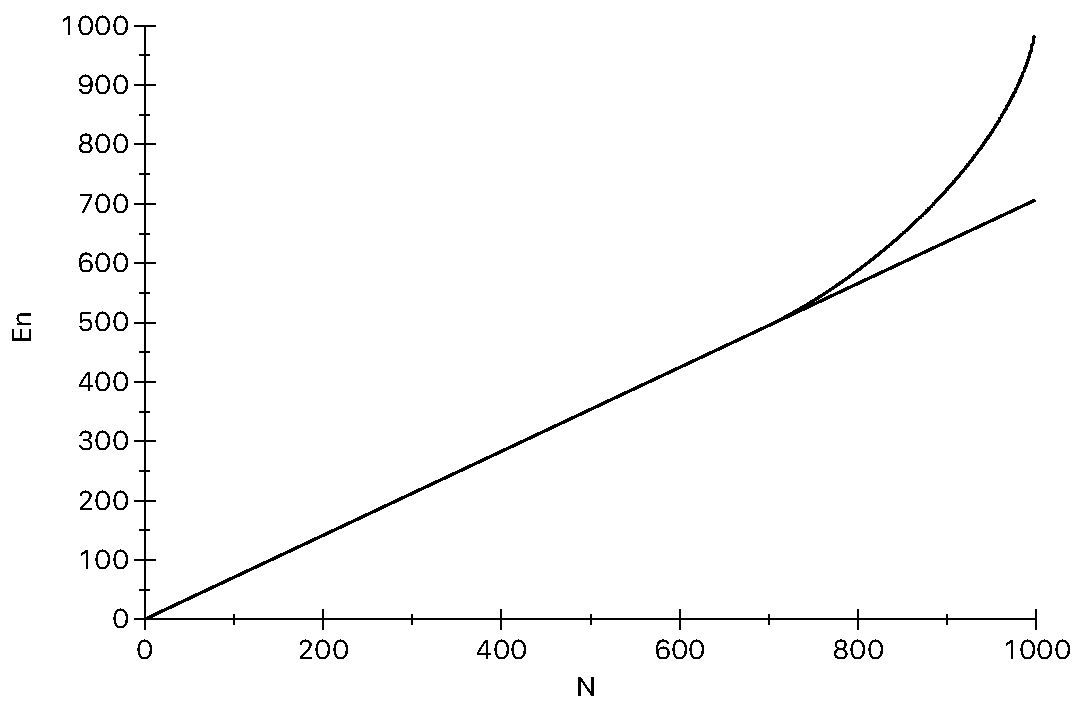
\includegraphics[width=13cm, height=8cm, angle=0]{w5.pdf}
			\caption{\label{Fig1} $\omega^2 = 0.5$. Explicit calculation is a straight line; Matrix interpretation curves upward}
	\end{figure}
	
	\begin{figure}[H]
		\centering
		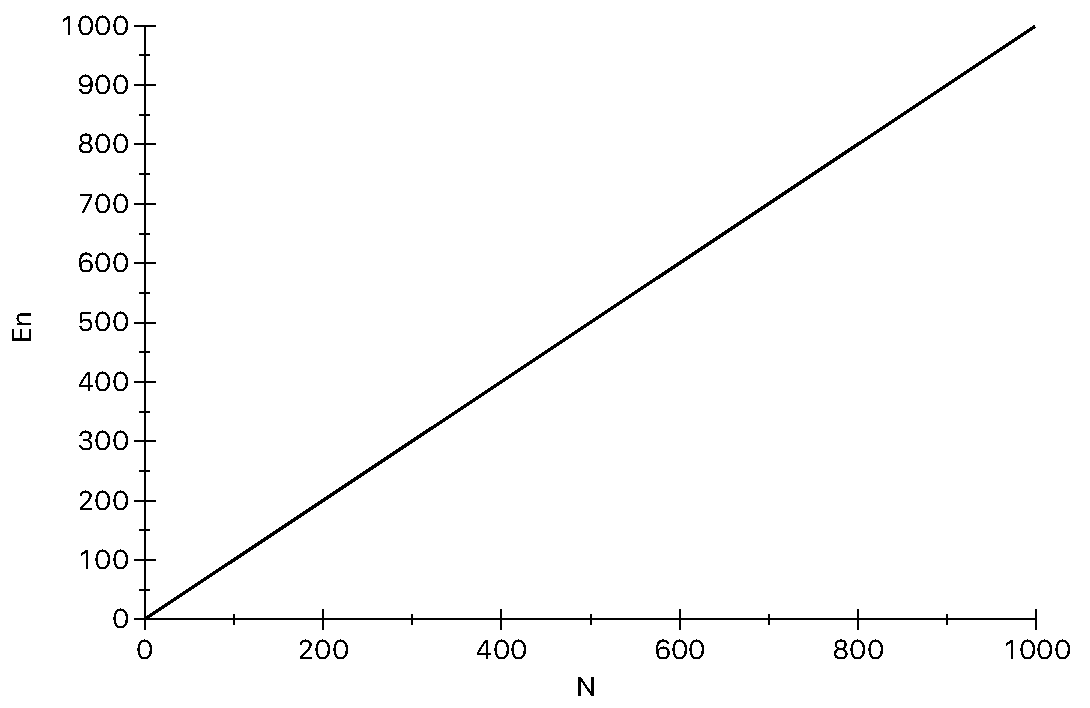
\includegraphics[width=13cm, height=8cm, angle=0]{w1.pdf}
			\caption{\label{Fig2} For $\omega^2 = 1$. Two lines lie on top of each other.}
	\end{figure}
	
	\begin{figure}[H]
		\centering
		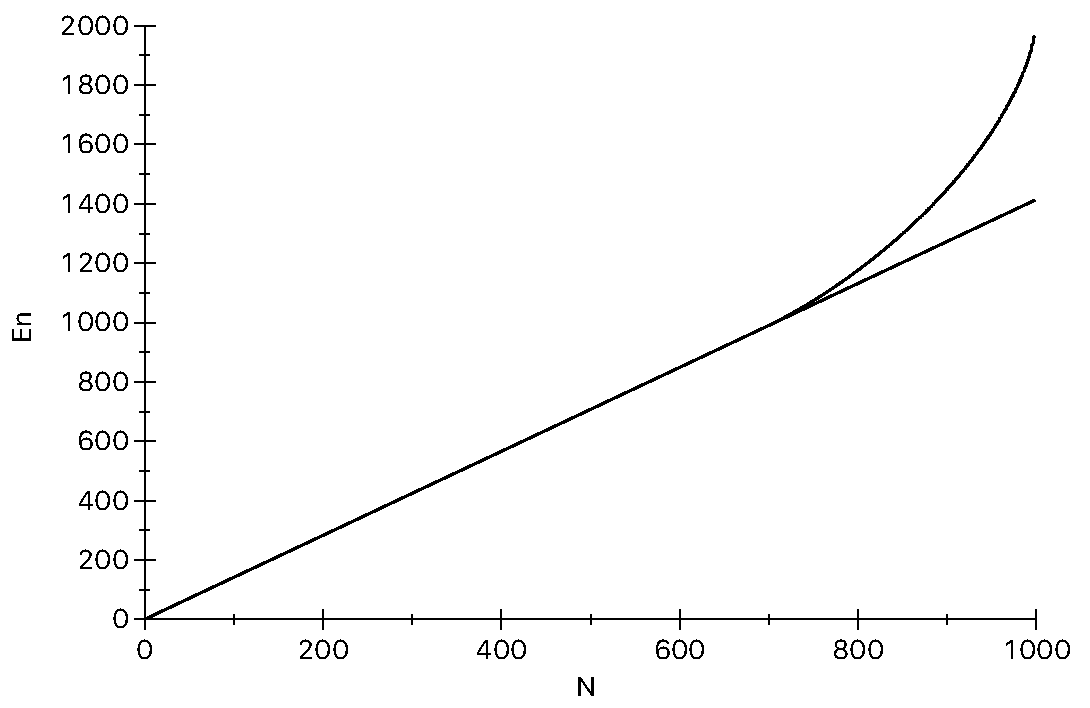
\includegraphics[width=13cm, height=8cm, angle=0]{w2.pdf}
			\caption{\label{Fig3} For $\omega^2 = 2$. Explicit calculation is a straight line; Matrix interpretation curves upward.}
	\end{figure}
	
	\begin{figure}[H]
		\centering
		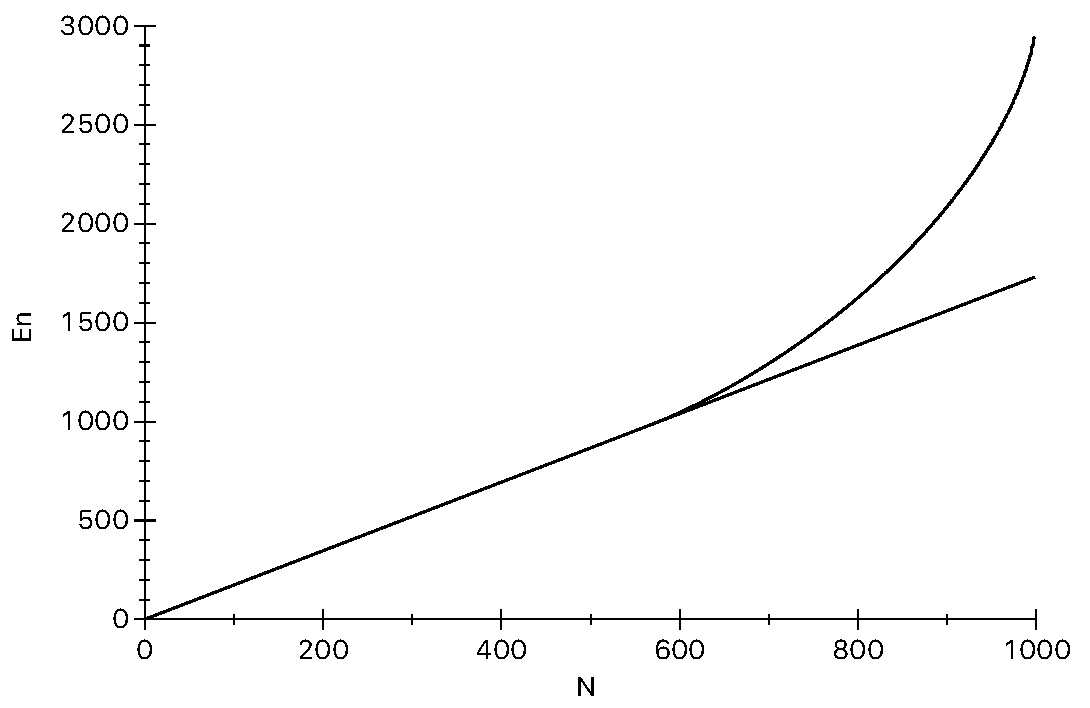
\includegraphics[width=13cm, height=8cm, angle=0]{w3.pdf}
			\caption{\label{Fig4} For $\omega^2 = 3$. Explicit calculation is a straight line; Matrix interpretation curves upward.}
	\end{figure}

After analysis, the orientation of the lines is a telling sign of the form of matrix (eigenvalues) that each $\omega^2$ iterates. We see that for  $\omega^2= 1$ the real eigenvalues of both calculations are consist, however this is not the case for the other $\omega^2$ values. In printing out a smaller matrix of these eigenvalues is clear as to why, while the $\omega^2$ for both explicit and matrix methods align themselves to the diagonals and as a result match numerically. The entries for  $\omega^2$ = .5, 2, and 3 do not, and as the dimension of the matrices increase in size the error of the matrix interpretation (intrinsic function) grows as well. The eigenvalues behavior interestingly occurs around the same place in all 3 cases, becoming divergent at around N=600...800.

\begin{thebibliography}{}

	\bibitem{}
	Z.~Papp and A.~Bill, {\it Computational Physics Lecture Notes}, California State University Long Beach.
	
\end{thebibliography}



\end{document}
